

\section{The 3.25 $\AA$ Peak } \label{Peak}
	To be able to detect a phase transition we first need to be able to detect a peak and characterize its features. In this section we describe how to characterize a peak. In particular, we will look at the peak located between 3.2 and 3.3 ${\AA}$.
	We characterize a peak by its center, width and area under it. To attribute these values for a given peak, we fit a gaussian function corrected for arbitrary area and background level. The unit area gaussian centered around $x_{0}$ with width $\sigma$ is given by eq. \ref{eq:gaus}
	\begin{equation} \label{eq:gaus}
	f(x) = \frac{1}{\sqrt{2\pi \sigma}} e^{-\frac{(x - x_{0})}{2\sigma^{2}} },
	\end{equation}
	
	We can add a constant background to this function by adding a constant $b$ and by multiplying $f(x)$ by A, we can interpret A as the area under the curve:
	\begin{equation} \label{eq:gausB}
	g(x) = Af(x) + b = \frac{A}{\sqrt{2\pi \sigma}} e^{-\frac{(x - x_{0})}{2\sigma^{2}} } + b,
	\end{equation}
	
	As we will see, this function is not a good hypothesis to fit peaks close to the phase transition temperature. The shape of those peaks are not gaussian at all, and a gaussian description is not adequate. A good way to evaluate how well the adopted function describes the data is to calculate the $\chi^{2}$ of the fit and look at the residues distribution. We are not implementing this analysis here. Mainly because we are actually not interested in the actual value of the area, or width of these peaks, but we are actually interested in finding a way to detect a phase transition. 
	Since the value of these variables will change drastically during a phase transition, this will actually be enough to detect it, so an accurate description of the shape of these peaks is not necessary. By using the function defined in \ref{eq:gausB} we have a very simple interpretation for our data and relatively fast algorithm that scales well with size.
	Figure \ref{fig:fits} shows the fitted curve for T = 0 K and T = 150 K. We can see that far from a phase transition, the fit works fine, whereas close to the phase transition the fit fails. Nonetheless we can see that the fitted values for $A, x_{0} \textrm{ and } \sigma$ are very different which allows us to see something is going on at that temperature.
	Figure \ref{fig:peak3p25} shows the values of $A, x_{0}, \sigma$ and background levels as a function of temperature for the 3.25 $\AA$ peak. Also, we show the same curves normalized in figure \ref{fig:norm} for visualization purposes.
	We can clearly see an interesting structure around 150 K. In all variables, the pattern followed by the curves is drastically changed by this phase transition.
	
	\begin{figure}[h]
	\centering
	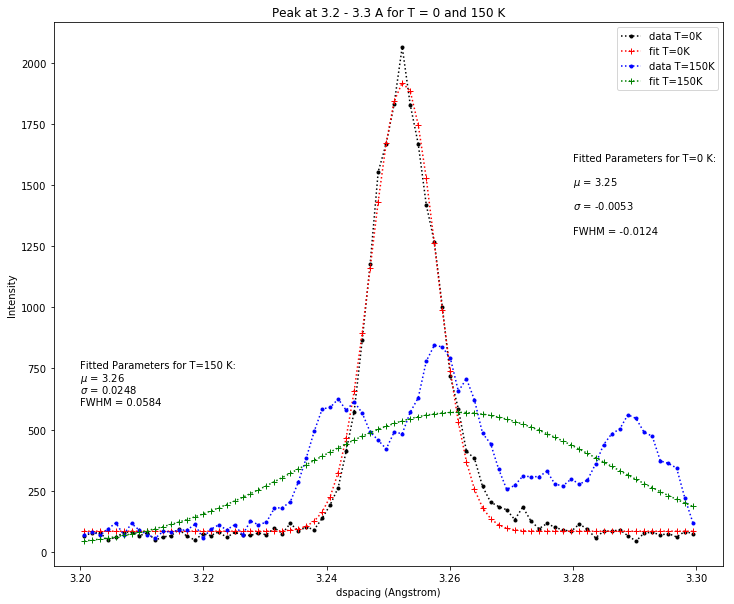
\includegraphics[scale=0.35]{../figs/fits.png}
	\caption{Gaussian fits for T = 0 and 150 K.}
	\label{fig:fits}
	\end{figure}
	
	\begin{figure}[h]
	\centering
	%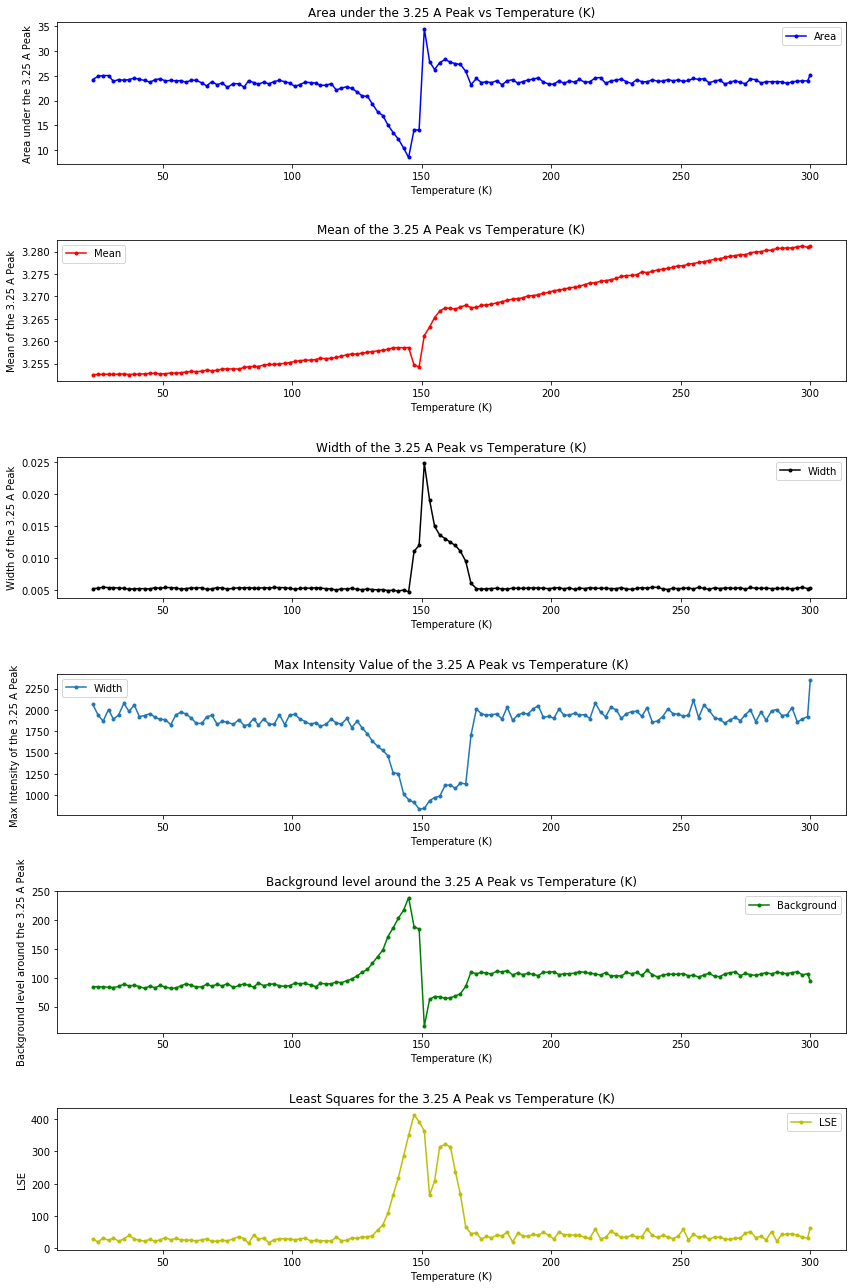
\includegraphics[width=0.8\linewidth, scale=0.25]{../figs/3p25.png}
	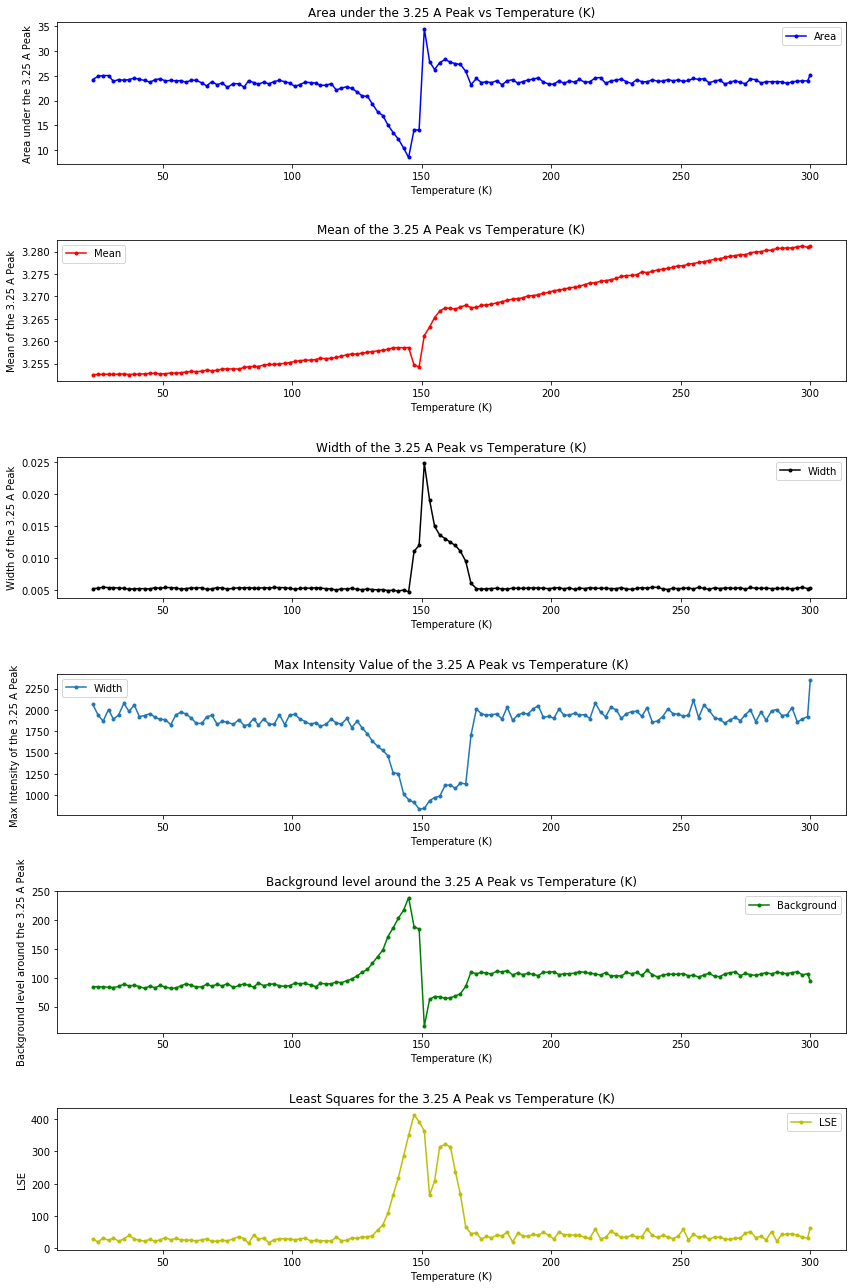
\includegraphics[scale=0.25]{../figs/3p25.png}	
	\caption{Area under the curve, center of the peak, peak width, maximum intensity, background level and chi2 of the fit as a function of temperature.}
	\label{fig:peak3p25}
	\end{figure}

	\begin{figure}[h]
	\centering
	%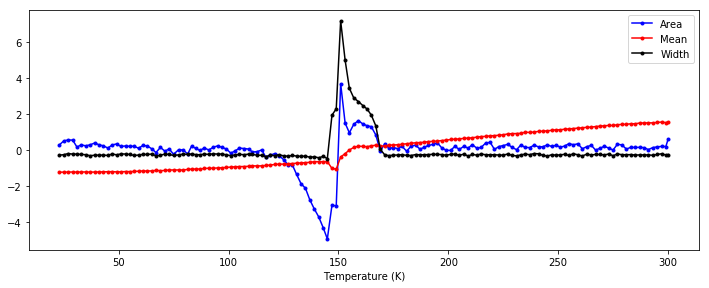
\includegraphics[width=0.8\linewidth]{../figs/norm.png}
	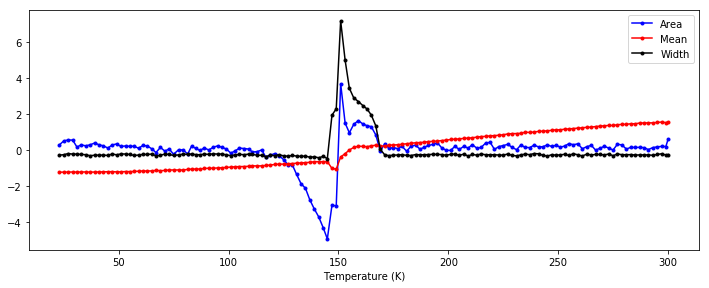
\includegraphics[scale=0.25]{../figs/norm.png}	
	\caption{Normalized area under the curve, center of the peak, peak width and background level as a function of temperature.}
	\label{fig:norm}
	\end{figure}
